\documentclass[12pt,a4paper]{article}

\usepackage[utf8]{inputenc}

\usepackage{varioref} % vref command
\usepackage[pdftex]{color,graphicx}
%\usepackage{natbib}
\usepackage[
    % ==========================================================================
    pdfauthor={
      Jiri Vinarek,
      Ondrej Fiala,
      Rudo Tomori,
      Viliam Simko (Supervisor)
    },
    pdftitle={Requirements Processing Tool},
    pdfsubject={Software project user-documentation},
    pdfkeywords={Use-cases, Formal methods, Model Checking},
    pdfproducer={Latex with hyperref},
    pdfcreator={pdflatex},
    % ==========================================================================
    pdfborder={0 0 0},
    unicode, % use UTF-8 for PDF properties
    plainpages=false,
    pdfpagelabels,
    hyperindex,
    hyperfigures=true,
    bookmarksnumbered=true, % generate section numbering in PDF bookmarks
    bookmarks,
    breaklinks=true, % allow URLs on multiple lines
    hypertexnames=true 
]{hyperref}

% must go after hyperref definition
\usepackage[all]{hypcap} % instead of captions, refs will scroll to images

\usepackage{url} % allow clickable URLs
\usepackage{graphicx}

\usepackage{framed} % frames around paragraphs
\usepackage{listings} % see http://en.wikibooks.org/wiki/LaTeX/Packages/Listings

\definecolor{DarkGray}{rgb}{0.3,0.3,0.3}
\definecolor{LightGray}{rgb}{0.6,0.6,0.6}
\definecolor{Green}{rgb}{0,0.6,0}
\definecolor{Purple}{rgb}{0.6,0,0.6}
\definecolor{Blue}{rgb}{0,0,1}

\hypersetup{colorlinks=true, linkcolor=black, urlcolor=black, citecolor=black}

\usepackage{pslatex} % times + courier monospace
%\usepackage{indentfirst}

%%%%%%%%%%%%%%%%%%%%%%%%%%%%%%%%%%%%%%%%%%%%%%%%%%%%%%%%%%%%%%%%%%%%%%%%%%%%%%%%
% NuSMV Input Language
%%%%%%%%%%%%%%%%%%%%%%%%%%%%%%%%%%%%%%%%%%%%%%%%%%%%%%%%%%%%%%%%%%%%%%%%%%%%%%%%
\usepackage{multicol}
\lstdefinelanguage{NuSMVLang}{
 ndkeywords={MODULE, VAR, INIT, ASSIGN, TRUE, FALSE, CTLSPEC, LTLSPEC, FAIRNESS, AX, A, AG, AF, U, boolean, next, case, esac, in},
 ndkeywordstyle=\color{Purple}\bfseries,
 identifierstyle=\color{black},
 sensitive=true,
 comment=[l]{--},
 morecomment=[s]{/*}{*/},
 commentstyle=\color{Green}\textit
}

%%%%%%%%%%%%%%%%%%%%%%%%%%%%%%%%%%%%%%%%%%%%%%%%%%%%%%%%%%%%%%%%%%%%%%%%%%%%%%%%
% Xtext Grammar
%%%%%%%%%%%%%%%%%%%%%%%%%%%%%%%%%%%%%%%%%%%%%%%%%%%%%%%%%%%%%%%%%%%%%%%%%%%%%%%%
\lstdefinelanguage{XtextGrammar}{
 ndkeywords={hidden, grammar, with, import, generate, as, terminal, fragment},
 ndkeywordstyle=\color{Purple}\bfseries,
 identifierstyle=\color{black},
 sensitive=true,
 comment=[l]{//},
 morecomment=[s]{/*}{*/},
 commentstyle=\color{Green}\textit,
 stringstyle=\color{Blue},
 morestring=[b]',
 morestring=[b]" 
}

%%%%%%%%%%%%%%%%%%%%%%%%%%%%%%%%%%%%%%%%%%%%%%%%%%%%%%%%%%%%%%%%%%%%%%%%%%%%%%%%
% Common design for all source codes
%%%%%%%%%%%%%%%%%%%%%%%%%%%%%%%%%%%%%%%%%%%%%%%%%%%%%%%%%%%%%%%%%%%%%%%%%%%%%%%%
\lstset{
 language=NuSMVLang,
 basicstyle=\scriptsize\sffamily,
 tabsize = 4,
 columns=fullflexible,
 numberstyle=\tiny\sffamily,
 %extendedchars=true,
 breaklines=true,
 %frame=bt,
 %framerule=2pt,
 numbers=left,
 %xrightmargin=3pt,
% framextopmargin=40pt,
% framexbottommargin=4pt,
 xleftmargin=16pt,
 framexleftmargin=16pt,
 morecomment=[l]{//},
% belowskip=15pt,
% aboveskip=10pt,
 mathescape=true,
 %linewidth=\textwidth,
 showstringspaces=false
}

\usepackage{amsthm}
\newtheorem{definition}{Definition}

% \newenvironment{definition}[1][Definition]{
% 	\setlength{\itemsep}{0cm}
% 	\setlength{\parskip}{0cm}
% 	\begin{trivlist}
% 	\item[\hskip \labelsep {\bfseries Definition: #1}]
% 	\item
% }{\end{trivlist}}

%\usepackage{setspace}
%\onehalfspacing

%\usepackage{fancyhdr} % vlastni podoba zahlavi/zapati
%\pagestyle{fancy}
%\fancyhead[L]{}
%\fancyhead[C]{\thepage}
%\fancyhead[R]{}

%% mene roztahane seznamy
%\usepackage{tweaklist}
%\renewcommand{\enumhook}{\setlength{\topsep}{4pt}%
%  \setlength{\itemsep}{0pt}}
%\renewcommand{\itemhook}{\setlength{\topsep}{4pt}%
%  \setlength{\itemsep}{0pt}}

\widowpenalty=10000 % zabrani vdovam (prvni radek odstavce na predchozi strane)
\clubpenalty=10000 % zabrani sirotkum (posledni radek odstavce na nove strane)

	\renewcommand\labelitemi{\normalfont\bfseries --}

\title{
  \textbf{Requirements Processing Tool}\\
  \vspace{26pt}
\includegraphics[height=5cm]{images/reprotool-logo}\\
  \vspace{16pt}\textbf{Software project user-documentation}
}

\author{
  Jiří Vinárek,
  Ondřej Fiala,
  Rudo Tomori
  \vspace*{120pt}
  \\Supervisor: Viliam Šimko
}

\date{\small{\today}}

\begin{document}
\maketitle
%\vspace{3cm}\abstract{The aim is to create a tool that allows users to bind requirements with the code of a developed application. Besides general requirements, the tool will semi-automatically process use-cases written in natural language. The idea is to reuse the algorithms and linguistic tools from the successful Procasor Environment project and to integrate them with the Eclipse platform.}
\thispagestyle{empty} % titulni strana bez cisla strany

\newpage

\tableofcontents
\vspace{12pt}

%\newpage

\section{Introduction}

% software development - elicitation
When developing a software application, analysts together with end-users negotiate properties of the intended system. This process involves elicitation of user requirements ranging from use-cases to non-functional properties.

% textual use-cases
A substantial part of the intended behaviour can be captured by writing textual use-cases which have the advantage of being able to address a wide range of stakeholders \cite{Larman,Cockburn:2000:WEU:517669}. Use-cases became a part of the UML standard \cite{UML-standard} and have since been greatly extended, being nowadays a mandatory requirement for any object-oriented software development project.

% drawbacks
On the other hand, the drawback of textual use-cases is the inherent vagueness and error-proneness of natural language. It is usually up to the developers to transform sentences to code and implement all the business parts of the system properly. Developers have to identify business entities and sequences of actions invoked by these entities. When coded manually, there is a high chance that the intended behaviour of a system does not correspond to the behaviour of a running application.

% solution
One of the possible approaches to minimizing such human errors is the model-driven development paradigm \cite{MDD} where automatic transformations between models are employed. However, before any transformation can be used, formal models have to be constructed first. In case of textual use-cases, this can be achieved in a semi-automatic way with the support of existing natural language processing (NLP) tools.

\subsection{Goals}
Reprotool is an IDE (Integrated Development Environment) providing software developers with tools to capture requirements of a developed system and to verify consistency of the system's specification. In the current version, Reprotool focuses on functional requirements in a form of  use-cases\footnote{Future versions will also support other types of requirements.}.

The tool allows users to interactively derive formal specification of the system's behavior from textual use cases. This way, both "user-readable" textual specification and precise formal specifications of the system is developed at the same time, only slightly increasing the effort required to write the use case models. The developed model can be further processed e.g. verified for consistency or exported to other formats, such as UML diagrams.

\subsection{History}
Based on the simple and uniform sentence structure used in textual use cases \cite{Cockburn:2000:WEU:517669}, a conversion scheme has been proposed in \cite{MenclDeriving,MenclImprovedDeriving} and later implemented in the Procasor Environment project. With the support of readily available NLP tools, Procasor Environment supported a semi-automatic transformation into a simple process algebra called \emph{Behaviour Protocols}~\cite{BehaviourProtocols}.

Reprotool has been greatly inspired by Procasor's way of handling natural language.
However, instead of the \emph{Behaviour Protocols}, Reprotool uses LTS (Label Transition System) as a formal description of the behaviour expressed by use-cases. Morover, Reprotool allows developers to verify consistency of that model using a state-of-the art symbolic model checker NuSMV~\cite{NuSMV-CAV02}.
\section{Manually creating a new \emph{Reprotool} project}

In this section we will walk through the process of creating a new simple \emph{Reprotool} project named \emph{PostOffice}.
Here, we are going to create the project manually. You will not need the project that we are creating here in the later parts
of this documentation. The chapter following this chapter deals with importing use-cases into \emph{Reprotool} project.
All exercises in this documentation will be based on the project from the next chapter, not this one.

\subsection{\emph{PostOffice} project description}
We will create a simple \emph{PostOffice} project that describes how a letter is written and then taken to the post office.
Our simple project will contain three use-cases and two actors. The \emph{PostOffice} project contains these use-cases:

\begin{enumerate}
 \item {\bf buyEnvelope}
 \item {\bf writeLetter}
 \item {\bf takeLetter}
\end{enumerate}

The \emph{PostOffice} project has these two actors specified:

\begin{enumerate}
 \item {\bf Peter} He writes the letter.
 \item {\bf officer} He works at the post office.
\end{enumerate}

\subsubsection{The \emph{buyEnvelope} use-case}

This use-case has the following structure:

\begin{enumerate}
 \item Peter goes to the shop
 \item Peter stands the queue
 \item Peter buys the envelope
 \item Peter goes home
\end{enumerate}

\subsubsection{The \emph{takeLetter} use-case}
\begin{enumerate}
 \item Peter goes to the post office
 \item Peter stands the queue
 \item Peter becomes impatient

 The queue has more than 10 people:
 \begin{enumerate}
  \item Peter goes home.
 \end{enumerate}


 \item The post officer takes the letter from Peter.
\end{enumerate}


\subsubsection{The \emph{writeLetter} use-case}
\begin{enumerate}

 \item Peter looks at his watches.

    Peter does not have enough free time:
    \begin {enumerate}
      \item Peter does something more important.
    \end {enumerate}

 \item Peter writes the letter.

 \item Peter checks if he has a spare envelope.
    
    Peter does not have a spare envelope:
    \begin {enumerate}
      \item Peter leaves the building.
      \item Include use-case buyEnvelope.
    \end {enumerate}

 \item Peter opens the envelope.

 \item Peter puts the letter into the envelope and closes it.
\end{enumerate}

\subsection{Create a \emph{Reprotool} project}
Create a new \emph{Reprotool} project using the command
\begin{verbatim}
 File / New / Reprotool Project
\end{verbatim}

A \emph{new project} dialog fires up. Enter the project name \emph{postOffice} and press \emph{Enter}. The new \emph{postOffice}
\emph{Reprotool} project has been created. You can view it now in the \emph{Project Explorer}. Now the \emph{project editor} has
started and we can start editing our (now empty) project.

The first thing we are going to do is to add actors to our project. You add actors by clicking the green \emph{plus} sign above the
\emph{Actors} field in the \emph{project editor}. Now please add the two actors to our project.

\subsection{Add use-cases to our project}
Now we are going to add the use-cases to our project. We will describe the process in greater detail for the use-case
\emph{writeLetter}. You add a use-case by clicking the \emph{plus} sign above the Use-cases field of the \emph{Project editor}.
After clicking on the \emph{plus} sign, the \emph{Use-case} editor has started. Now we are going to edit the use-case.

Firstly, enter the use-case name \emph{writeLetter} and think of a suitable \emph{description} of the use-case.
Then select the \emph{Peter} as the \emph{primary actor} of the use-case.

Now it is time to add the individual use-case steps to our use-case. Notice that the use-case by default already contains one single
use-case step. You add other steps by right-clicking on use-case step and select the
\begin{verbatim}
New Sibling / Use Case Step
\end{verbatim}
 command. Now proceed by firstly adding the steps of the \emph{main scenario} only. That is, add the following steps to the use-case:

\begin{enumerate}
 \item Peter looks at his watches.
 \item Peter writes the letter.
 \item Peter checks if he has a spare envelope.
 \item Peter opens the envelope.
 \item Peter puts the letter into the envelope and closes it.
\end{enumerate}

Now we will add an \emph{extension scenario} to the use-case step 1 (Peter looks at his watches). An \emph{extension scenario} is an
ordered set of steps than can be attached to some use-case step. The steps of an extension scenario are executed \emph{after} the execution
of the associated step if the associated condition is met. So now right-click the first use-case step and select this command:
\begin{verbatim}
 New Child / Extensions scenario
\end{verbatim}
A new \emph{extension scenario} has been created. It has the label \emph{1a (ext.)} because it is attached to the use-case step with label
\emph{1}. The created scenario by default contains a single step. Enter this text in the use-case editor right next to the label
\emph{1a (ext.)}
\begin{verbatim}
Peter does not have enough free time:
\end{verbatim}
Then fill the single use-case step of our extension scenario with this text:
\begin{enumerate}
 \item Peter does something more important.
\end{enumerate}

Now create an extension scenario to the step three in a same way. But now attach this text to the extension scenario:
\begin{verbatim}
Peter does not have a spare envelope:
\end{verbatim}

Add a second step to the extension scenario so that it is 2 steps long. And fill the steps with this text:
\begin {enumerate}
 \item Peter leaves the building.
 \item Include use-case buyEnvelope.
\end {enumerate}

Now we are finished with the \emph{writeLetter} use-case. Proceed in a similar way and create the other two missing use-cases.
Select \emph{Peter} as the \emph{primary actor} of the use-case \emph{buyEnvelope} and select the \emph{Officer} as the primary actor
of the \emph{takeLetter} use-case.

In the following figure you can view the \emph{PostOffice} project while editing the \emph{takeLetter} use-case.

\begin{figure}[ht]
  \centering
  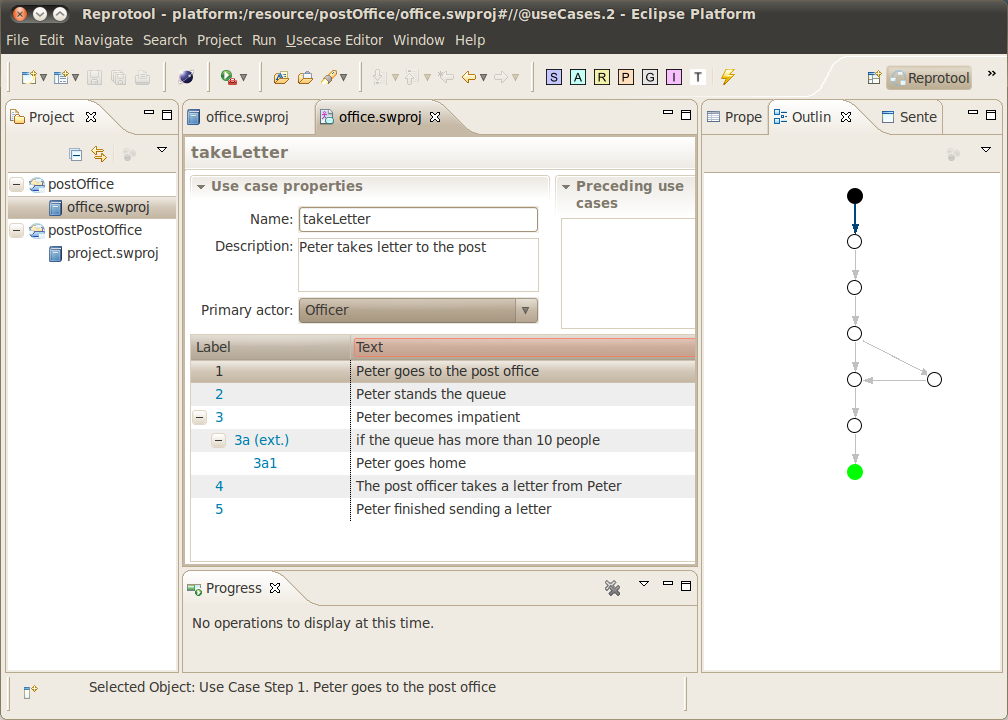
\includegraphics[height=280pt]{images/reprotoolUCEditor}
  \caption{\emph{takeLetter} use-case}
  \label{fig:reprotoolUCEditor}
\end{figure}

\newpage

\subsection{Add \emph{actions} to the use-case steps}

In this step we will need the \emph{Sentence Analysis} view. You can display it by this command:
\begin{verbatim}
 Window / Show View / Other
\end{verbatim}

and select \emph{Reprotool} from the dialog box that appears. Now click on the \emph{Sentence Analysis} and click OK. This should make
the \emph{SentenceAnalysis view} visible.

\subsubsection{\emph{Actions} in the \emph{writeLetter} use-case}

Now we will define the \emph{Abort} action for the only use-case step of the first step extension scenario. Click on the use-case step
with label \emph{1a1} and select \emph{Abort} as \emph{Action Type} in the \emph{Sentence Analysis View}. You can view this situation
in the next picture:

\begin{figure}[ht]
  \centering
  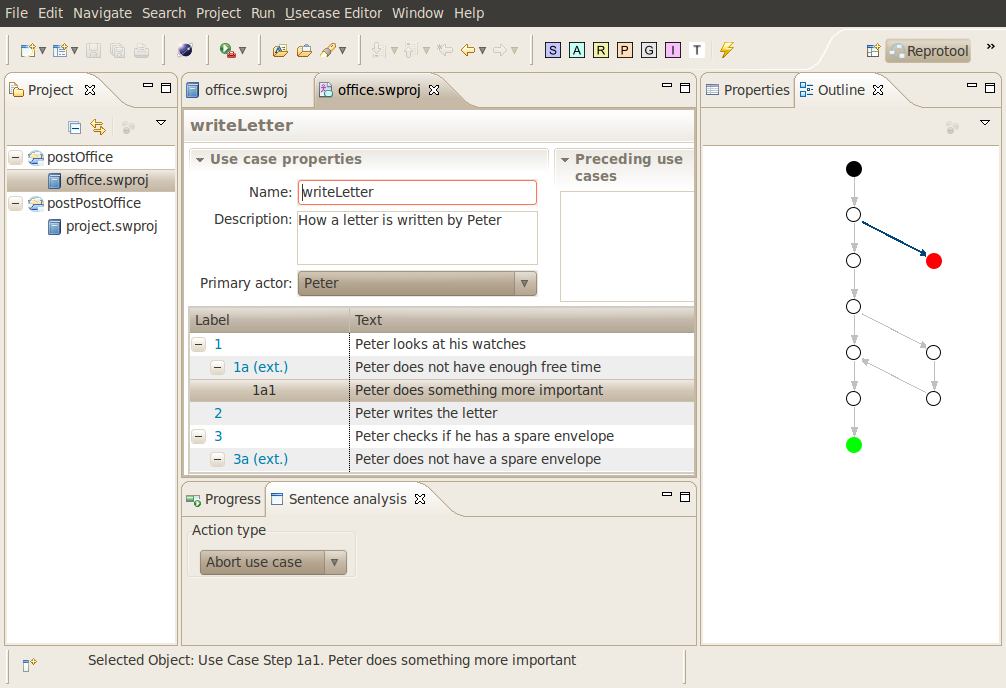
\includegraphics[height=280pt]{images/reprotoolAbort}
  \caption{\emph{Abort} use-case step action specified}
  \label{fig:reprotoolAbort}
\end{figure}

\newpage

Now we will define an \emph{include action} for the use-case step with label \emph{3a2}. So click this use-case step and in the
\emph{Analysis} view, select \emph{Use case include} as the action type and select the use-cese \emph{buyEnvelope} as the included
use-case. You can view the situation in the next picture. Also notice the outline view that shows also the included use-case schema. 

\begin{figure}[ht]
  \centering
  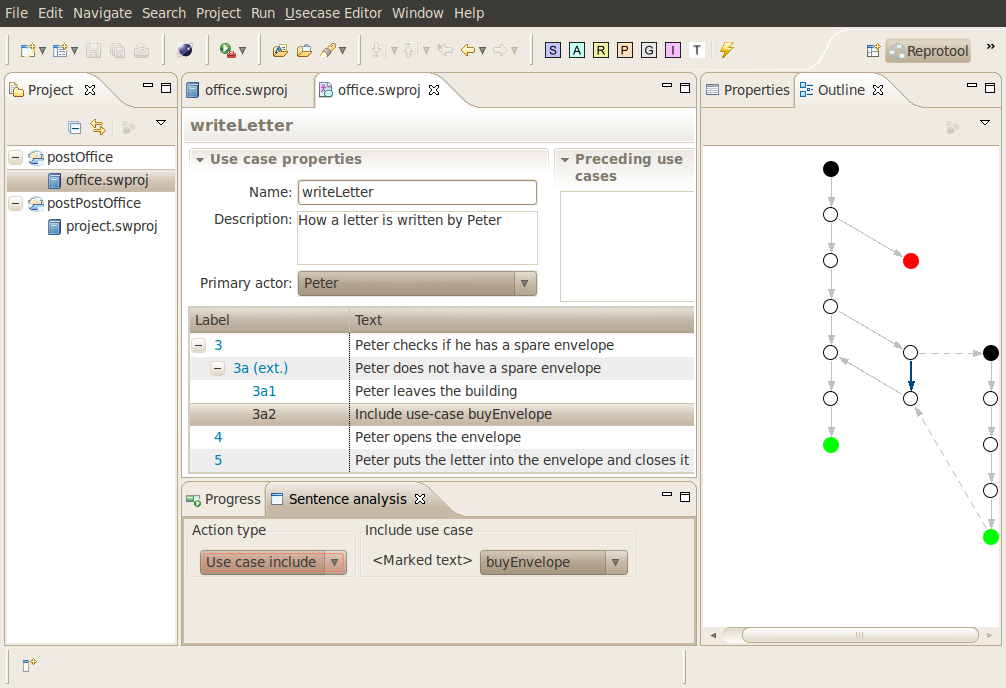
\includegraphics[height=280pt]{images/reprotoolInclude}
  \caption{\emph{Include} use-case step action specified}
  \label{fig:reprotoolInclude}
\end{figure}

\subsubsection{\emph{Actions} in the \emph{takeLetter} use-case}

Now, please specify the \emph{Abort} action for the use-case step labeled \emph{3a1} in the \emph{takeLetter} use-case. (The step text
reads: \emph{Peter goes home}).

\subsubsection{\emph{Actions} in the \emph{buyEnvelope} use-case}
There are no actions specified in this use-case.

\newpage

\subsection{Add \emph{annotations} to the use-case steps}

In this step we will need the \emph{Properties} view. If it is not displayed, you can show it with this command:
\begin{verbatim}
 Window / Show View / Properties
\end{verbatim}

Now we will add \emph{annotations} to some of the use-case steps. The newly created \emph{Reprotool} project already contains a vocabulary
of annotations that are ready to be used. We will now show how to use them.

\subsubsection{\emph{Annotations} in the \emph{writeLetter} use-case}
The second use-case step of this use-case reads: \emph{Peter writes the letter}. We will add an annotation of
type \emph{create} to this step. Right-click on this step in the use-case editor. Execute this command:
\begin{verbatim}
 New Child / StepAnnotation
\end{verbatim}
A new \emph{Annotation} will be created under the specified use-case step. Now look at the \emph{Properties view} and select
\emph{create} as annotation type. Write \emph{letter} as annotation id. Notice in the \emph{Properties view}, that \emph{Reprotool}
automatically generates an annotation \emph{description} by concatenating the annotaion \emph{type} and the annotation \emph{id}.
In this case it reads \emph{\#create\_letter}.
Also notice that in the \emph{OutlineView} the annotated use-case steps have a small violet square drawn over them. You can view this
situation in the next figure:

\newpage

\begin{figure}[ht]
  \centering
  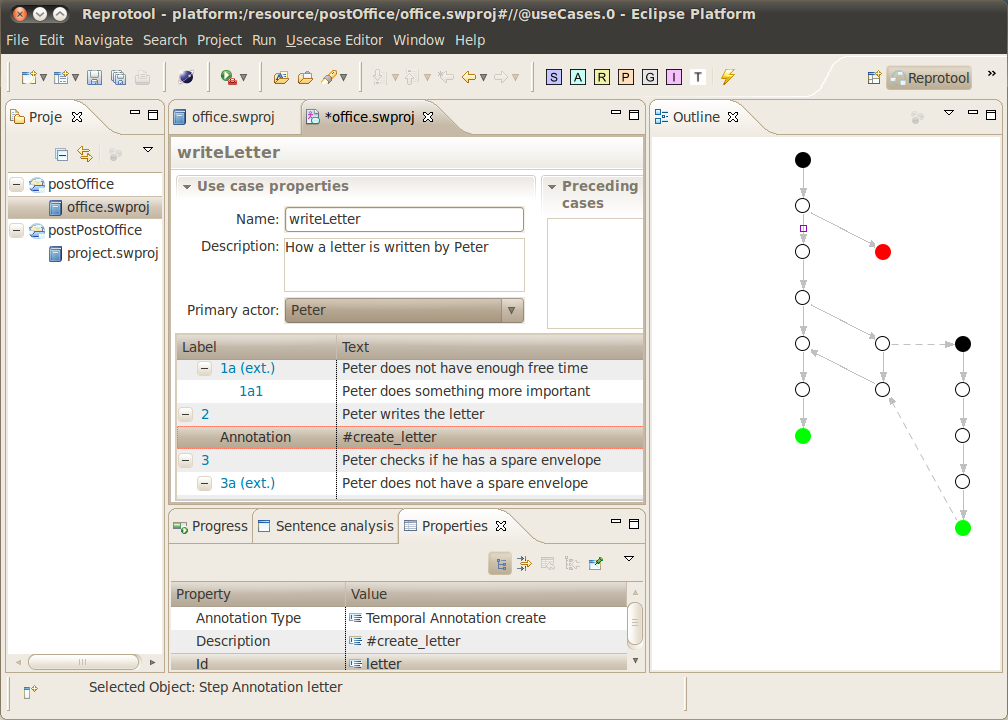
\includegraphics[height=280pt]{images/reprotoolAnnot}
  \caption{\emph{create} annotation specified}
  \label{fig:reprotoolAnnot}
\end{figure}

Now add the annotation \emph{\#open\_envelope} to the step \emph{Peter opens the envelope} and add annotation \emph{\#close\_envelope}
to the step \emph{Peter puts the letter into the envelope and closes it}.

\subsubsection{\emph{Annotations} in the \emph{takeLetter} use-case}
Please add the annotaion \emph{\#create\_letter} to the step in use-case \emph{takeLetter} that reads: \emph{Peter goes home}\footnote{Please don't be worried if you think this annotation does not belong here. Indeed, it doesn't. But we create it
here just to show in the later part of this tutorial what happens when you break the semantics of annotations.}.
Also add the annotaion \emph{\#use\_letter} to the step in the same use-case that reads: \emph{The post officer takes the letter
from Peter}.

\subsubsection{\emph{Annotations} in the \emph{buyEnvelope} use-case}
There are no annotations in this use-case.

\newpage

\subsection{Specify \emph{precedence relations} between use-cases.}

We will now add a precedence relation between use-cases \emph{writeLetter} and \emph{takeLetter} specifying that the use-case
\emph{takeLetter} can be executed only after the use-case \emph{writeLetter} successfully finished. Open now the use-case
\emph{takeLetter} in the use-case editor. Click on the icon in the \emph{Preceding use-cases} area. A dialog box now appears that
allows you to specify preceding use-cases of the use-case \emph{takeLetter}. Now select the \emph{writeLetter} use-case in the left part
of the dialog window and click the \emph{add} button to copy this use-case to the right part of the window. Then just press OK. This
situation is depicted in this figure:

\begin{figure}[ht]
  \centering
  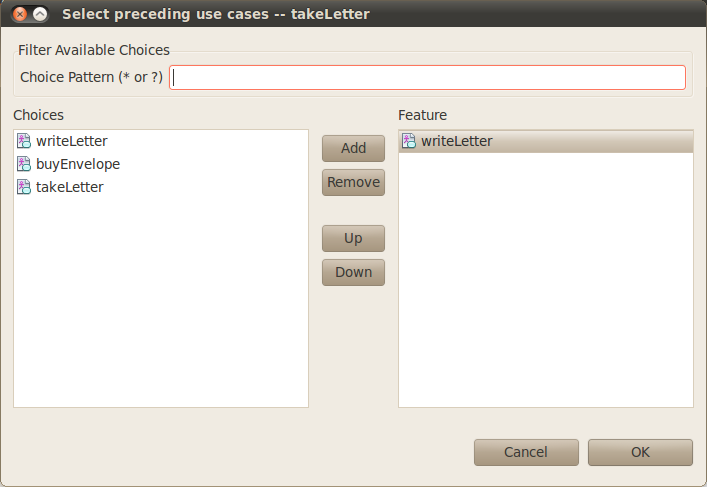
\includegraphics[height=280pt]{images/reprotoolPrecede}
  \caption{\emph{precede} annotation specified}
  \label{fig:reprotoolPrecede}
\end{figure}
\section{Verification of consistency}

A software project specification can be verified for consistency within Reprotool.
This section provides details about the verification process.

The system's behaviour is specified by the set of use-cases contained within the project.
Use-cases and their relations are stored in a memory structure we refer to as a use-case model (Figure~\ref{fig:ReprotoolUCModel}).
The model is based on the EMF framework so that it integrates well within the Eclipse environment.

\begin{figure}[ht]
  \centering
  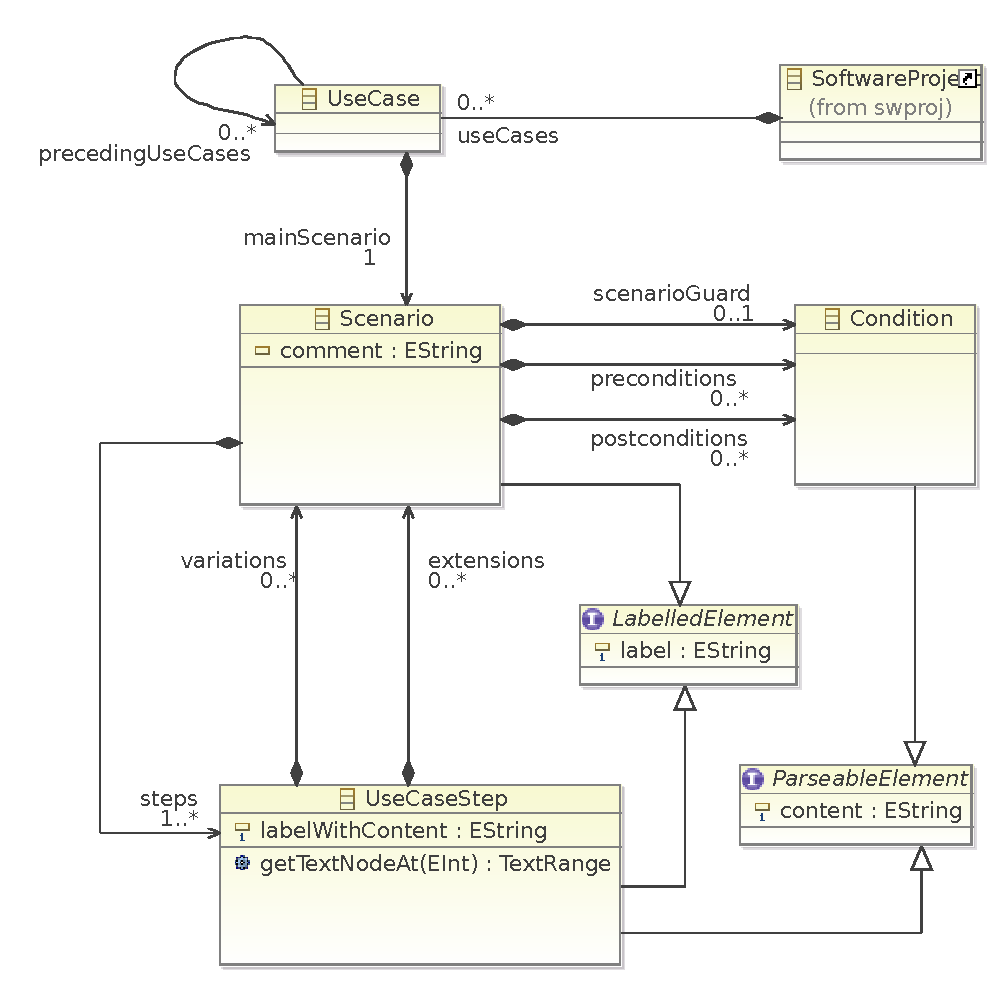
\includegraphics[width=280pt]{images/ReprotoolUCModel}
  \caption{Use-case model}
  \label{fig:ReprotoolUCModel}
\end{figure}

\subsection{Annotations model}

When we refer to verifying the consistency of a system, we actually consider the consistency of temporal properties implied by the annotations used within the project.

Every reprotool project contains a set of temporal constraints imposed upon annotations in the project.
Annotations\footnote{An intuitive example of annotations is the annotation pair \emph{open-close}. For such annotations we could describe constraints like \emph{After open there should always be close}, or \emph{No multi open without close}.} can be attached to individual use-case steps (see \emph{StepAnnotation} element depicted in Figure~\ref{fig:ModelOfAnnotations}).


An annotation attached to a use-case step consists of two parts\footnote{An example of an annotation type we use in Reprotool is \emph{open}.
A suitable \emph{id} for annotation of this type could be \emph{file1}, thus the description of this annotation reads \textcolor{Blue}{\emph{open\_file1}}.}
-- \emph{type} and \emph{id}.

\begin{figure}[ht]
  \centering
  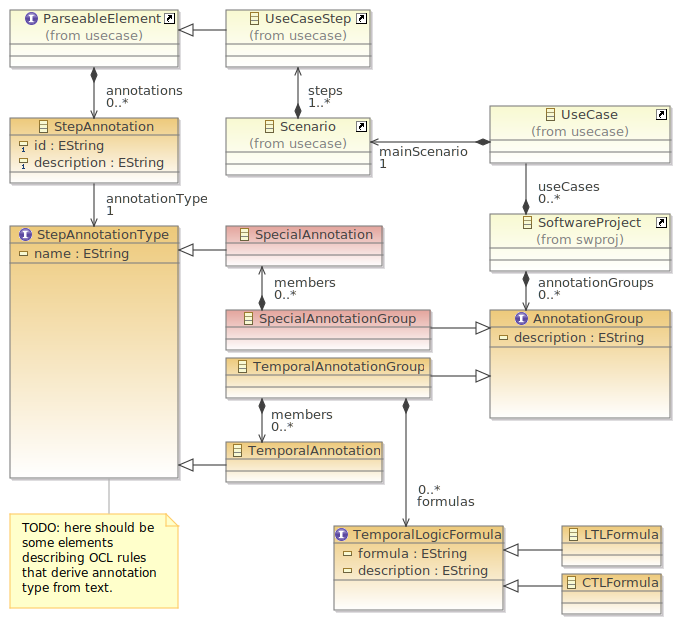
\includegraphics[width=\textwidth]{images/ReprotoolUCAnnotModel}
  \caption{Model of annotations}
  \label{fig:ModelOfAnnotations}
\end{figure}

Every reprotool project specifies a "vocabulary" of annotations (i.e. types of annotations) that users can use to annotate use-case steps. When assigning a \emph{StepAnnotation} to a given step, users would combine \emph{StepAnnotationType} with an arbitrary \emph{id}.

Annotations are organized in groups as depicted in Figure~\ref{fig:ModelOfAnnotations}. Currently, Reprotool supports two kinds of annotations:
\begin{description}

	\item[Temporal annotations] organized in \emph{TemporalAnnotationGroup}s, whose semantics is specified by a set of temporal logic formulae; their format will be described later on.
	
	\item[Special annotations] organized in \emph{SpecialAnnotationGroup}s, whose semantics is hard-coded in Reprotool.
\end{description}

\subsection{Special annotations}

When a \emph{reprotool} user creates a new project from the \emph{Eclipse IDE} new project wizard, a special \emph{trace-on} annotation group is added to the project.
This annotation group contains two special annotations -- \emph{trace} and \emph{on}.
Currently, these are the only special annotations supported by \emph{Reprotool}.
These two special annotations enable the users to select mutually exclusive paths in their use-case scenarios.
This might be used to prune the computation tree the \emph{NuSMV} tool considers when checking the \emph{CTL}/\emph{LTL} specifications.

Let's assume we have a use-case \emph{U} that has the main scenario 7 steps long.
Step 1 and the step 4 have both an extension scenario 3
steps long.
The individual use-case steps are annotated as depicted in the following picture:


\begin{figure}[ht]
  \centering
  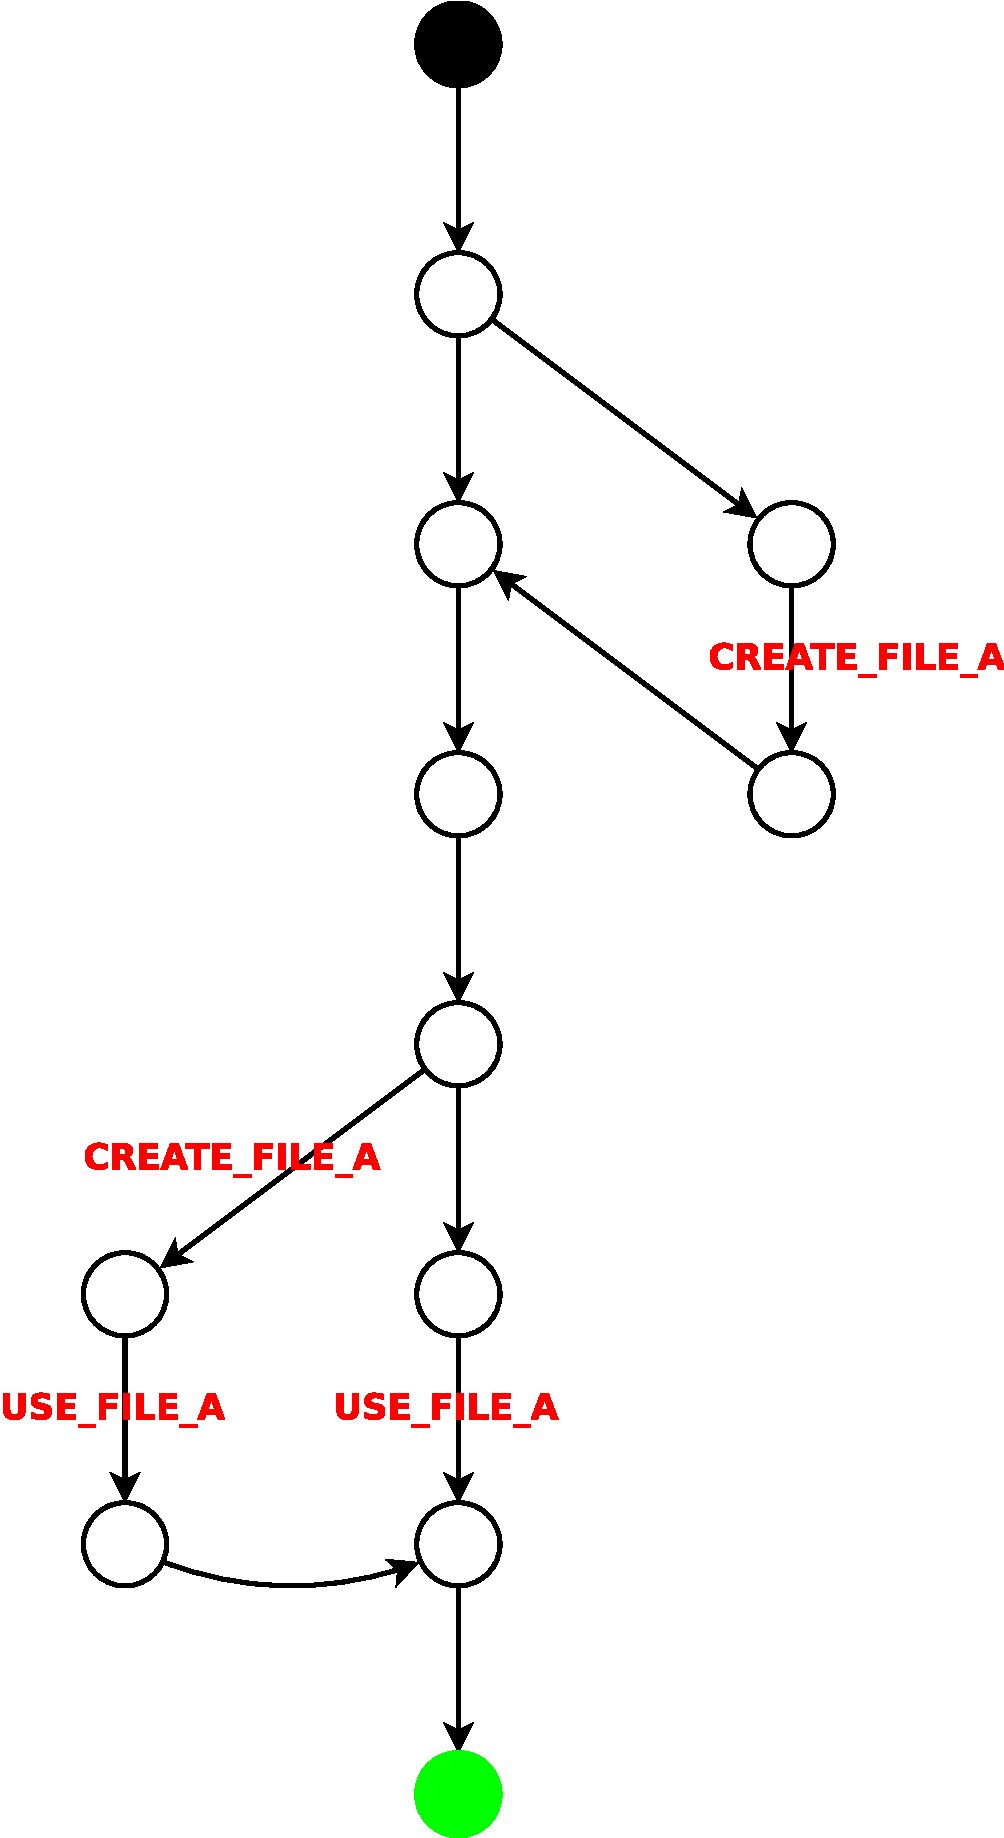
\includegraphics[width=180pt]{images/traceTest_no_trace}
  \caption{Schema of the use-case \emph{U}}
  \label{fig:traceTest_no_trace}
\end{figure}


The use-case \emph{U} contains two annotation types -- \emph{create} and \emph{use}.
One of the constraints imposed on such annotations is a CTL formula:
\begin{verbatim}
CTLSPEC AG( create -> AX(AG(!create)) ) -- Only one 'create'
\end{verbatim}

That means you cannot create a given object more than once.
However, looking at the use-case \emph{U} carefully, it is obvious that there is an execution path containing  the annotation \textcolor{red}{\emph{CREATE\_FILE\_A}} twice.

To solve the problem in the previous example, user needs to specify that if the first extension scenario has been taken, then the second extension scenario of use-case step 4 can not be taken. On the other hand, if the first extension scenario has not been taken,
then the second extension scenario must be taken.
And this is exactly what the \emph{trace} and \emph{on} annotations are for.

\begin{definition}[Semantics of the trace-on annotation pair]
	Let $S$ be a a use-case step.
	Let $on\_x$ be an annotation attached to $S$ (\emph{x} is and arbitrary annotation id).
	Let $T=\{t: S \in t\}$ be a set of all traces going through the step $S$.
	A trace $t \in T$ will be considered for verification only if it contains a step $R'$ annotated with $trace\_x$ before the step $S$.
\end{definition}

Let's clarify it with the help of an example.
In the Figure~\ref{fig:traceTest} you can see the same use-case \emph{U} but with properly added
\emph{trace} and \emph{on} annotations that prevent any conflicts.

\begin{figure}[ht]
  \centering
  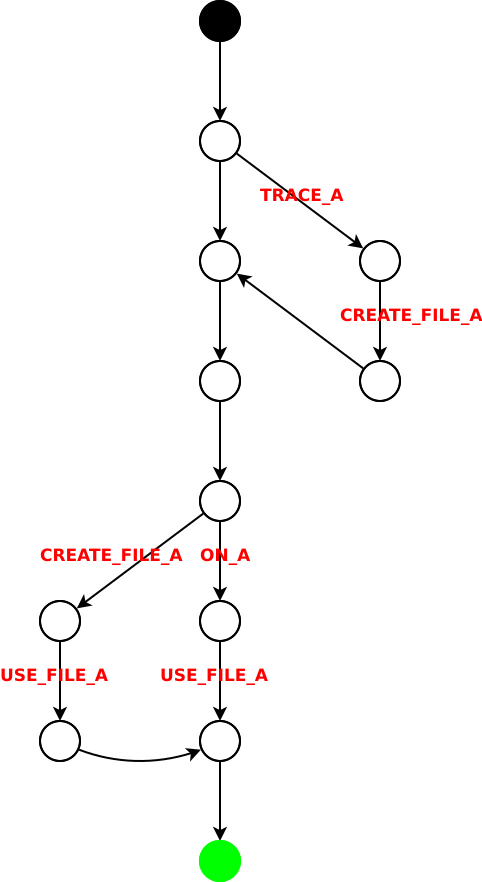
\includegraphics[width=180pt]{images/traceTest}
  \caption{Schema of the use-case \emph{U} with trace/on annotations added}
  \label{fig:traceTest}
\end{figure}

The annotated use-case \emph{U} has now only two execution paths possible. And none of them violates any of the default constraints
imposed on the \emph{create} and \emph{use} annotations. Here you can see the path where the \emph{trace}/\emph{on} branch has been
taken:

\begin{figure}[ht]
  \centering
  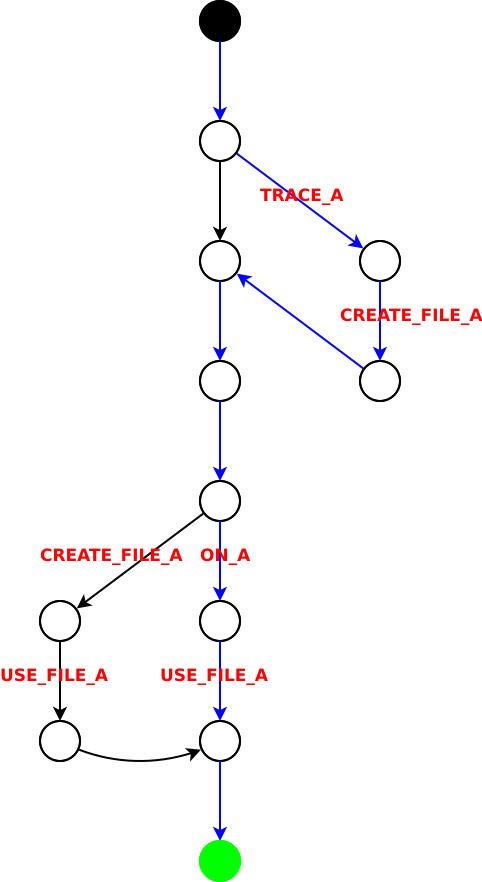
\includegraphics[width=180pt]{images/traceTest_path_taken}
  \caption{\emph{Trace}/\emph{on} branch taken}
  \label{fig:traceTestTaken}
\end{figure}

When the \emph{NuSMV} tool simlates the execution of the state machine corresponding to the annotated use-case \emph{U} and just finished
execution of the 4 step of the use-case main scenario, there would normally by 2 possibilities how to proceed. But because in our
example execution path the \emph{trace\_a} annotaion has been encountered, there is only one possibility - and that is to take the
\emph{on} branch.

\newpage

The situation where the second path has been taken is depicted in the next picture. No other execution paths are considered by the
\emph{NuSMV} tool.

\begin{figure}[ht]
  \centering
  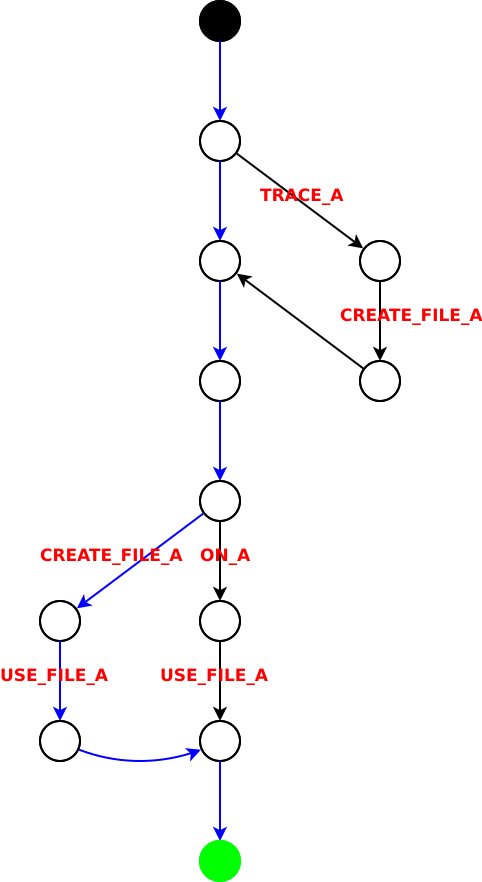
\includegraphics[width=180pt]{images/traceTest_path_not_taken}
  \caption{\emph{Trace}/\emph{on} branch NOT taken}
  \label{fig:traceTestNotTaken}
\end{figure}

\subsection{NuSMV symbolic model checker}

We use NuSMV~\cite{NuSMV-CAV02,NuSMV-frocos02} symbolic model-checker to verify consistency of use-cases with regard to their temporal annotations.
Although NuSMV support BDD-based\footnote{Using binary decision diagrams} and BMC-based\footnote{Bounded model-checking using a SAT solver} model-checking techniques, in our project we use just the BDD-based approach.
NuSMV supports analysis of synchronous and asynchronous systems using Computation Tree Logic (CTL) and Linear Temporal Logic (LTL).
Our framework supports both CTL and LTL, however CTL is preferred because NuSMV would convert LTL formulae into CTL internally (as described in \cite{NuSMV-ltl-fmsd97}).

All use-cases from our UC model have to be converted into NuSMV input language.
We use Xtext\cite{Xtext-website} as a tool for handling DSLs (Domain Specific Languages) which in this case is the NuSMV input language.

NuSMV input language is described using EBNF grammar (inspired by \cite{googlecode-nusmv-tools}) and Xtext generates:
\begin{itemize}
  \item an in-memory representation of the parse tree, sometimes being referred to as an Abstract Syntax Tree (AST),
  \item a text-to-AST parser and
  \item a AST-to-text serializer
\end{itemize}

In order to convert our UC model into NuSMV input language, we use the model-to-model (M2M) approach.
We traverse the UC model and during that traversal we collect the neccesary information to build a new EMF memory structure based on the generaetd NuSMV model.
The generated serializer then produces a valid NuSMV code from the NuSMV model.

\begin{figure}[ht]
  \centering
  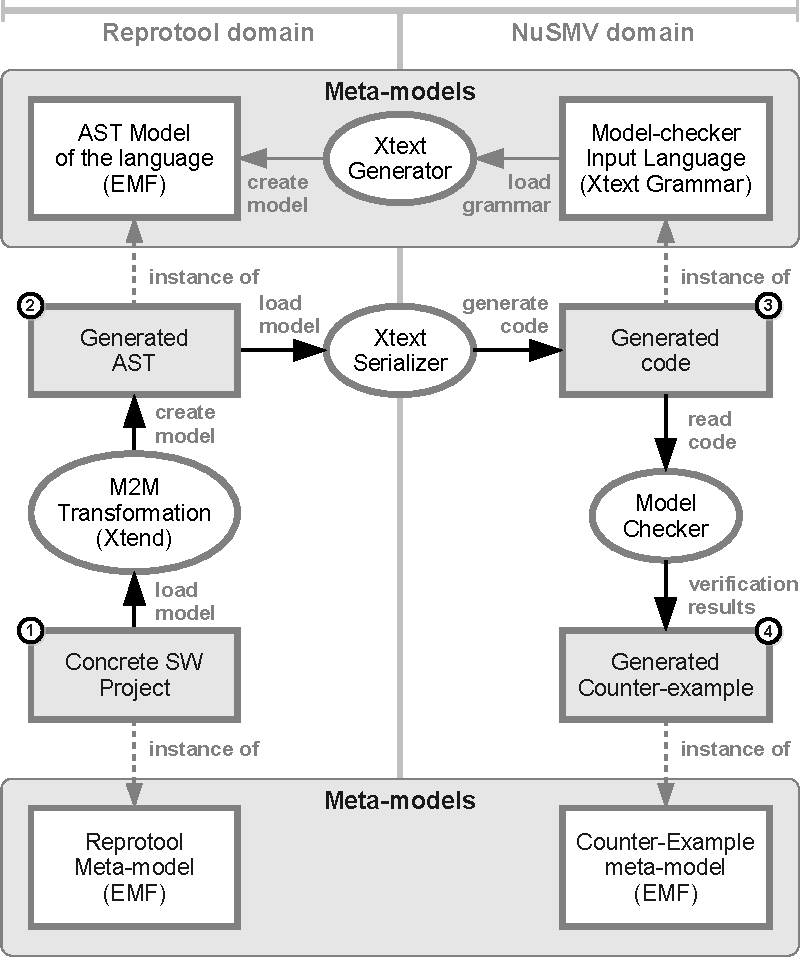
\includegraphics[height=280pt]{images/XtextWorkflow}
  \caption{Transformation of a SW Project into the input language of a model checker}
  \label{fig:XtextWorkflow}
\end{figure}
\pagebreak

\subsection{NuSMV temporal logic formulas}

Temporal annotations of a reprotool project are organised in \emph{TemporalAnnotationGroups}. (See Figure~\ref{fig:ModelOfAnnotations}.)
Every \emph{TemporalAnnotationGroup} contains a set of logically grouped temporal annotations and a set of \emph{temporal logic formulas}
that specify the semantics of the temporal annotations in the group. The NuSMV tool and Reprotool support two types of temporal logic
formulas. And that is:

\begin{enumerate}
 \item CTL (Computation Tree Logic) formulas
 \item LTL (Linear Temporal Logic) formulas
\end{enumerate}

\subsubsection{CTL formulas}
Specify format of CTL formulas

\subsubsection{LTL formulas}
Specify format of LTL formulas

\subsection{Generated NuSMV model}

The NuSMV language model is based on the EMF framework and is generated from the NuSMV language grammar.
This model describes the classes that build up the AST (Abstract Syntax Tree) of the NuSMV language.

Here we present an excerpt from the NuSMV language grammar. You can find the whole grammar in th
\emph{reprotool.fm.nusmv.lang} plugin in the \emph{NuSMVLang.xtext} file.

\begin{lstlisting}[language=XtextGrammar]
grammar reprotool.fm.nusmv.lang.NuSmvLang with org.eclipse.xtext.common.Terminals
generate nuSmvLang "http://d3s.mff.cuni.cz/reprotool/nusmv/lang"
import "http://www.eclipse.org/emf/2002/Ecore" as ecore

Module:
	"MODULE" (MainModule | OtherModule)
	(moduleElement+=ModuleElement)*;
MainModule:
	name='main';

OtherModule:
	name=ID ("(" (params+=FormalParameter) ("," params+=FormalParameter)* ")")?;

ModuleElement hidden(WS, SL_COMMENT):
	  VariableDeclaration
	| IVariableDeclaration
	| FrozenVariableDeclaration
	| DefineDeclaration
	| ConstantsDeclaration
	| AssignConstraint
	| TransConstraint
	| InitConstraint
	| InvarConstraint
	| FairnessConstraint
	| CtlSpecification
	| LtlSpecification
	| InvarSpecification
;
\end{lstlisting}

The Xtext generates an EMF model from the specified grammar. You can have a hierarchical view of the generated model by displaying the
\emph{NuSMVLang.ecore} file in the \emph{reprotool.fm.nusmv.lang} plugin. To better visualise the model, right-click on the \emph{NuSMVLang.ecore} file in
the package explorer of the Eclipse IDE and click the option ``Initialize Ecore Diagram file...''. This will create the \emph{NuSMVLang.ecorediag} file that you can view with the provided Eclipse editor.

% TODO: tento obrazok nesuvisi s textom. Treba ho vyhodit?
\begin{figure}[ht]
  \centering
  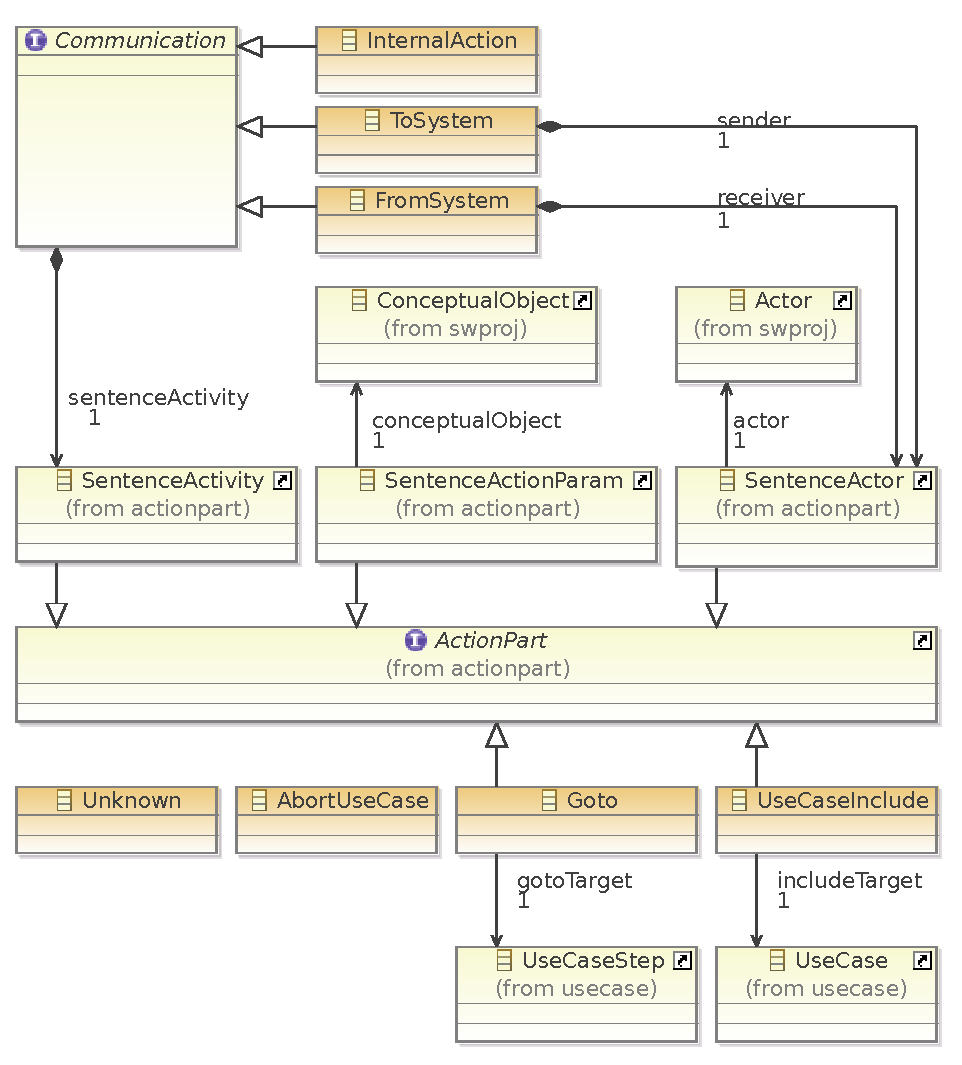
\includegraphics[width=260pt]{images/ReprotoolActionsModel}
  \caption{Model of derived action}
  \label{fig:ReprotoolActionsModel}
\end{figure}

\subsection{Model to model transformation}

Here we present an overview of the transformation of our UC model into the generated NuSMV model. The objective of this process is to take a reprotool project as input and transform it into the generated NuSMV model.

All transformations are implemented using the Xtend~\cite{Xtend-website} language.
Xtend is a statically-typed programming language which is compiled to Java and therefore integrates well and runs on JVM. It brings many concepts simplifying model-to-model and model-to-text transformation. We have leveraged on the following Xtend features: 
\begin{itemize}
	\item Advanced type inference
	\item Extension methods - enhance closed types with new functionality.
	\item Closures - concise syntax for anonymous function literals.
		These features are used for implementing the builder design pattern.
	
		\verb|$(...factory code...)[...initialization code...]|
	
	\item Multiple dispatch a.k.a. polymorphic method invocation.
	\item Operator overloading (e.g. \verb|map += key -> value|)
	\item Property access syntax - shorthands for getter and setter access.
\end{itemize}

This transformation is implemented in the \emph{reprotool.fm.nusmv} plugin in the \emph{reprotool.fm.nusmv.mapping} package.
The transformation itself is quite straight-forward and is defined in an Xtend class \emph{NuSMVProj.xtend}.
For every use-case we create a definition of a non-deterministic state machine.
The state machine's states are directly related to the steps of the related use-case.
The use-cases in the reprotool project can have precedence relations specified. Theses relations are considered in the
transformation process. The use-case state machines are instantiated with a parameter that triggers the execution of the machine.
With this parameter we ensure that the precedence relations are fulfilled. By means of this parameter we also avoid parallel execution
of multiple use-cases.

One part of this model transformation process is to generate NuSMV CTL/LTL formulas which are to be checked by the NuSMV tool. The
skeletons of these formulas are provided by the user in the reprotool project. In this model to model transformation process these
formula skeletons are simply expanded by substituting the annotation patterns with annotations found in the steps of the use-cases
in the reprotool project. A detailed example with explanation is provided in the next section.

\subsection{Example of a reprotool project converted into NuSMV}

In this section we present a simple reprotool project consisting of two use-cases. We show by the means of an example how this project
gets transformed into the NuSMV language format.

The project contains two use-cases. For every use-case U one state machine M is generated. This machine is represented by the states and
transitions between them that are derived directly from the use-case steps of the use-case U. Let's assume our project contains a use
case U1. The use-case U1 has a main scenario that contains five use-case steps. Use-case step 1 is annotated by the annotation \emph{open\_file}
and use-case step 2 is annotated by the annotation \emph{close\_file}. Step 2 has two extension scenarios (One is three steps and the other
one two steps long) and step 4 has one extension scenario two steps long. Step 4 includes another use-case U2 from the project. The
main scenario of use-case U2 contains only single step. You can have a look at the visual representation of the use-case U1 (and also
use-case U2 since it is included in the step 4 of the main scenario of the use-case U1) in the following figure. The initial state is
filled with black colour and the final state is filled with green colour. Steps 1 and 2 are marked with a violet square because these
steps are annotated.

\begin{figure}[h]
  \centering
  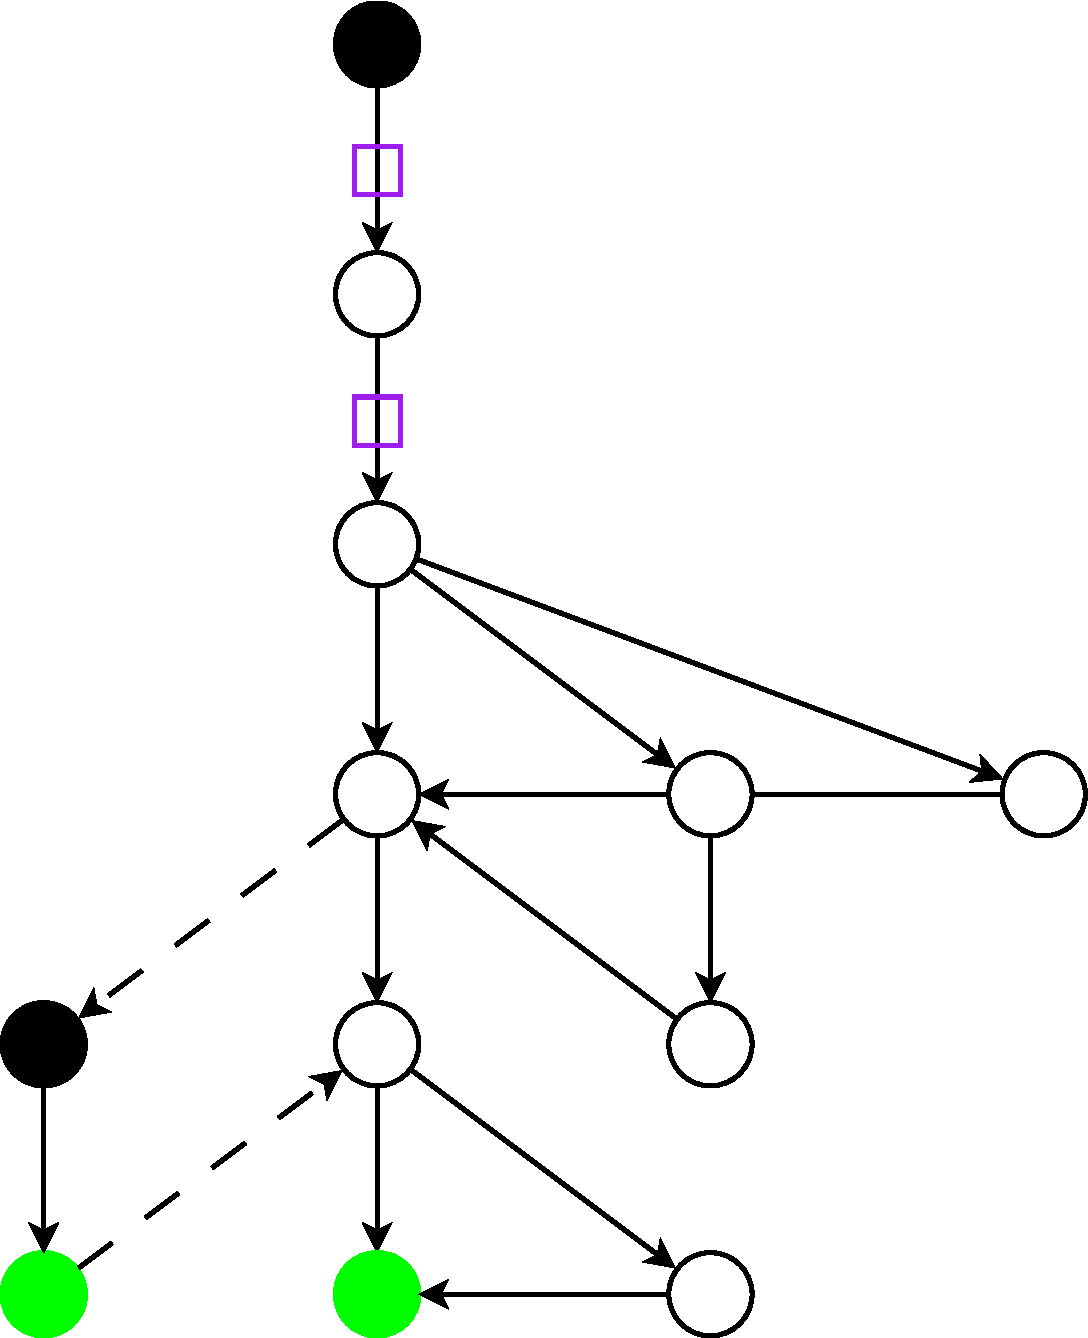
\includegraphics[width=200pt]{images/u1}
  \caption{Visual representation of the use-case U1}
  \label{fig:use-case U1}
\end{figure}

Now we present the state machine M that represents the use-case U1 and is written down using the NuSMV syntax. The state machine is
represented by a single module UC\_U1. This module contains a definition of variable s to which values representing variour machine
states can be assigned. Indeed, the transition to state s1 in the state machine is simulated by assigning the value s1 to the
variable s. The biggest part of the module UC\_U1 specification takes up a case construct that specifies various state transitions
of the machine based on the current state. Becuase use-case U1 includes another use-case U2 (which is represented by the module
UC\_U2), the module UC\_U1 also contains a variable y1 that is an instantiation of the module UC\_U2 included in the module UC\_U1.
\begin{lstlisting}
MODULE UC_U1 ( top , run )
	VAR y1run : boolean ;
	INIT y1run in FALSE
	VAR y1 : UC_U2 ( top , y1run ) ;
	ASSIGN next ( y1run ) := (s=s3__) ;
	VAR s : { s0 , s_ext_3 , s_ext_2 , s2 , s1 , s3__ , s2a2 , s3_ , s2_ , s2b1 ,
		s3a1 , s1_ , s2a1 , s3 , sFin } ;
	INIT s in s0
	ASSIGN next ( s ) := case
		s=s0 & !run : s0;
		s=s0 & run : {s1_};
		s=s3__ & y1.s != sFin : s3__;
		s=s3__ & y1.s  = sFin : s3_;
		s=s_ext_2 : {s3__};
		s=s2 : {s2a1,s2b1,s_ext_2};
		s=s1 : {s2_};
		s=s2a2 : {s_ext_2};
		s=s3_ : s3;
		s=s2_ : s2;
		s=s2b1 : {s_ext_2};
		s=s3a1 : {s_ext_3};
		s=s1_ : s1;
		s=s2a1 : {s2a2};
		s=s3 : {s3a1,s_ext_3};
		s=s_ext_3 : sFin;
		s=sFin : sFin;
	esac ;
\end{lstlisting}

Here we present the machine M2 that represents the included use-case U2.
\begin{lstlisting}
MODULE UC_U2 ( top , run )
	VAR s : { s0 , s1 , sFin } ;
	INIT s in s0
	ASSIGN next ( s ) := case
		s=s0 & !run : s0;
		s=s0 & run : {s1};
		s=s1 : sFin;
		s=sFin : sFin;
	esac ;
\end{lstlisting}

As we have already mentioned when describing use-case U1, the first two steps of its main scenario are annotated. (This is denoted
by a small violet square in the graphical representation of the use-case U1). Every such an annotation generates an annotation variable
definition in the NuSMV model. The variable name encodes the annotation type (for example open) and the annotation id (for example
file1). The variable is of boolean type and is initialized with the logical value of zero. The variable value is set to logical one
if and only if the state variable s of the respective state machine module denotes that the machine is in the annotated state.

Let's clarify this a bit more with the example of our project. There we have use-case step one of the use-case U1 annotated with the
open annotation (annotation id is file1) and step two annotated with the close annotation (annotation id is file1). These two use-case
step annotations in the use-case U1 of our project yield the following annotation variable definitions:

\begin{lstlisting}
VAR open_file1 : boolean ;
INIT open_file1 in FALSE
ASSIGN next ( open_file1 ) := FALSE
	| xU1.s in {s1_} ;
VAR close_file1 : boolean ;
INIT close_file1 in FALSE
ASSIGN next ( close_file1 ) := FALSE
	| xU1.s in {s2_} ;
\end{lstlisting}

Now we will describe the variable named \emph{p} which has the function of a steering wheel of whole simulation performed by the \emph{NuSMV} tool
when looking for possible violations of our system. This variable is of type enum and can assume the value \emph{none}, or other n values that
map directly to the n use-cases present in our project. The \emph{p} variable is initialised with the \emph{none} value. When the \emph{NuSMV} tool performs
steps in our system which are basicly transitions in the state machines of our use-cases, the value of the \emph{p} variable alternates between
the \emph{none} value and any other value from the set of possible values. Thus, the \emph{p} variable definition looks like this:
\begin{lstlisting}
VAR p : { none , pU1 , pU2} ;
INIT p in none
ASSIGN next ( p ) := case
	p=none : {pU1, pU2};
	TRUE : none;
esac ;
\end{lstlisting}

The \emph{p} variable helps us to decide which state machine could be executed in the next steps. We also generate definition for the
boolean variable \emph{idle} that tells us if any of the use-case state machines is currently being executed. The \emph{idle} variable is defined
by the means of a set of boolean variables from which every variable tells us if the machine to which it maps is currently
being executed. This is how it looks in the \emph{NuSMV} syntax:
\begin{lstlisting}
VAR idle : boolean ;
INIT idle in TRUE
ASSIGN next ( idle ) := case
	xU1run | xU2run : FALSE;
	TRUE : TRUE;
esac ;
\end{lstlisting}

Next we need to define for every use-case \emph{UN} a boolean variable \emph{xUNrun} that triggers the execution of the respective state machine
and at the same time serves as an indicator if the respective state machine N is currently running. This boolean variable is
initialised with logical zero. It is assigned the logical one only if all other machines are idle and the p variable points to the
machine N. For every use-case UN we also need to define a variable \emph{xUN} that is the actual instantiation of the state machine N.
Of course this variable is of type \emph{UC\_UN}. This is how the definitions of the variables \emph{xUN} and \emph{xUNrun} look in practice:
\begin{lstlisting}
VAR xU1 : UC_U1 ( self , xU1run ) ;
VAR xU1run : boolean ;
INIT xU1run in FALSE
ASSIGN next ( xU1run ) := case
	p=pU1 & idle & xU1.s = s0 : TRUE;
	TRUE : xU1run & xU1.s != sFin;
esac ;
\end{lstlisting}

Now we are going to describe how the \emph{CTL} and \emph{LTL} specifications are generated. When a new empty reprotool project is generated in the
\emph{Eclipse IDE}, it already contains a set of predefined \emph{CTL} formulas along with a quick description of each formula. Here is a subset of
these predefined formulas that is relevant to the \emph{open}/\emph{close} annotations:

\begin{description}
 \item [$AG(open \rightarrow AF(close))$] After 'open' there should always be 'close'
 \item [$AG(open \rightarrow AX(A\lbrack!open \cup close\rbrack))$] No multi-open without close
 \item [$AG(close \rightarrow AX(A\lbrack!close \cup open \mid !AF(close) \rbrack))$] No multi-close without open
 \item [$A\lbrack !close \cup open \mid !AF(close)\rbrack$] First 'open' then 'close'
\end{description}

We can see that these logical formulas specify properties for the open and close annotations. We also know that in the use-case \emph{U1} we
use annotation \emph{open\_file1} and \emph{close\_file1}. Now we simply expand the predefined \emph{CTL} and \emph{LTL} formulas. This is what we get in our
example:
\begin{lstlisting}
CTLSPEC AG(open_file1 -> AF(close_file1))
CTLSPEC AG(open_file1 -> AX(A[!open_file1 U close_file1]))
CTLSPEC AG(close_file1 -> AX(A[!close_file1 U open_file1 | !AF(close_file1) ]))
CTLSPEC A[!close_file1 U open_file1 | !AF(close_file1)]
\end{lstlisting}

And this is what the \emph{NuSMV} file looks like:
\begin{lstlisting}
MODULE main
	CTLSPEC AG(open_file1 -> AF(close_file1))
	CTLSPEC AG(open_file1 -> AX(A[!open_file1 U close_file1]))
	CTLSPEC AG(close_file1 -> AX(A[!close_file1 U open_file1 | !AF(close_file1) ]))
	CTLSPEC A[!close_file1 U open_file1 | !AF(close_file1)]

	FAIRNESS p=pU1
	FAIRNESS p=pU2
	FAIRNESS p=pU3

	VAR p : { none , pU1 , pU2} ;
	INIT p in none
	ASSIGN next ( p ) := case
		p=none : {pU1, pU2};
		TRUE : none;
	esac ;

 	VAR idle : boolean ;
	INIT idle in TRUE
	ASSIGN next ( idle ) := case
		xU1run | xU2run : FALSE;
		TRUE : TRUE;
	esac ;

 	VAR xU1 : UC_U1 ( self , xU1run ) ;
	VAR xU1run : boolean ;
	INIT xU1run in FALSE
	ASSIGN next ( xU1run ) := case
		p=pU1 & idle & xU1.s = s0 : TRUE;
		TRUE : xU1run & xU1.s != sFin;
	esac ;

	VAR xU2 : UC_U2 ( self , xU2run ) ;
	VAR xU2run : boolean ;
	INIT xU2run in FALSE
	ASSIGN next ( xU2run ) := case
		p=pU2 & idle & xU2.s = s0 : TRUE;
		TRUE : xU2run & xU2.s != sFin;
	esac ;

 	VAR open_file1 : boolean ;
	INIT open_file1 in FALSE
	ASSIGN next ( open_file1 ) := FALSE
		| xU1.s in {s1_}
	;

	VAR close_file1 : boolean ;
	INIT close_file1 in FALSE
	ASSIGN next ( close_file1 ) := FALSE
		| xU1.s in {s2_}
	;

MODULE UC_U1 ( top , run )
	VAR y1run : boolean ;
	INIT y1run in FALSE
	VAR y1 : UC_U2 ( top , y1run ) ;
	ASSIGN next ( y1run ) := (s=s3__) ;
	VAR s : { s0 , s_ext_3 , s_ext_2 , s2 , s1 , s3__ , s2a2 , s3_ , s2_ , s2b1 ,
			s3a1 , s1_ , s2a1 , s3 , sFin } ;
	INIT s in s0
	ASSIGN next ( s ) := case
		s=s0 & !run : s0;
		s=s0 & run : {s1_};
		s=s3__ & y1.s != sFin : s3__;
		s=s3__ & y1.s  = sFin : s3_;
		s=s_ext_2 : {s3__};
		s=s2 : {s2a1,s2b1,s_ext_2};
		s=s1 : {s2_};
		s=s2a2 : {s_ext_2};
		s=s3_ : s3;
		s=s2_ : s2;
		s=s2b1 : {s_ext_2};
		s=s3a1 : {s_ext_3};
		s=s1_ : s1;
		s=s2a1 : {s2a2};
		s=s3 : {s3a1,s_ext_3};
		s=s_ext_3 : sFin;
		s=sFin : sFin;
	esac ;

MODULE UC_U2 ( top , run )
	VAR s : { s0 , s1 , sFin } ;
	INIT s in s0
	ASSIGN next ( s ) := case
		s=s0 & !run : s0;
		s=s0 & run : {s1};
		s=s1 : sFin;
		s=sFin : sFin;
	esac ;
\end{lstlisting}

 
\end{document}
